\subsection{SCARA robot}\label{sec:CtrlScara}
As a simple example of a multi-body system we consider a SCARA robot as displayed in \autoref{fig:Scara}.
For the sake of demonstration we neglect the vertical axis and the tool orientation.
The remaining two axis are sufficient to position a tool (red point in \autoref{fig:Scara}) in the workspace (green shaded area).

\begin{figure}[ht]
 \centering
 \input{graphics/Scara.pdf_tex}
 \caption{A Scara robot and its mechanical model (image \url{www.epson.com})}
 \label{fig:Scara}
\end{figure}

\paragraph{Model.}
The model consists of two rigid bodies constraint by two revolute joints.
A reasonable choice of coordinates are the relative joint angles $\sysCoord = [\jointAngle[1], \jointAngle[2]]^\top$ and their derivatives $\sysVel = [\jointAngled[1], \jointAngled[2]]^\top$.
The rigid body configurations are
\begin{subequations}
\begin{align}
 \bodyHomoCoord{0}{1} &=
 \begin{bmatrix}
  \cos\jointAngle[1] & -\sin\jointAngle[1] & 0 & 0 \\
  \sin\jointAngle[1] &  \cos\jointAngle[1] & 0 & 0 \\
  0 & 0 & 1 & 0 \\
  0 & 0 & 0 & 1
 \end{bmatrix},&
 \bodyJac{0}{1} &= \begin{bmatrix} 0 & 0 \\ 0 & 0 \\ 0 & 0 \\ 0 & 0 \\ 0 & 0 \\ 1 & 0 \end{bmatrix}
\\
 \bodyHomoCoord{1}{2} &=
 \begin{bmatrix}
  \cos\jointAngle[2] & -\sin\jointAngle[2] & 0 & l_1 \\
  \sin\jointAngle[2] &  \cos\jointAngle[2] & 0 & 0 \\
  0 & 0 & 1 & 0 \\
  0 & 0 & 0 & 1
 \end{bmatrix},&
 \bodyJac{1}{2} &= \begin{bmatrix} 0 & 0 \\ 0 & 0 \\ 0 & 0 \\ 0 & 0 \\ 0 & 0 \\ 0 & 1 \end{bmatrix}
 .
\end{align} 
\end{subequations}

% \autoref{tab:ScaraMdlParam} collects the relevant values inside the body inertia matrices $\bodyInertiaMat{0}{1}{}$, $\bodyInertiaMat{0}{2}{}$ \wrt to the chosen body fixed frames which will later be used for simulation.
% Remark that the joint axis are parallel to the gravity direction and consequently there are no gravitational forces.
% Overall we assume no potential $\potentialEnergy = 0$ and no dissipative influences $\sysDissMat = 0$.
% The only external force on the system are the control forces $\sysInput = [\tau_1, \tau_2]^\top$ that act on the joint axes.

% \begin{table}
% \centering
% \setlength\extrarowheight{1ex}
% \begin{tabular}{rc}
%  \toprule
%  length arm 1 & $l_1 = 0.3\,\unit{m}$ \\
%  length arm 2 & $l_2 = 0.2\,\unit{m}$ \\
%  mass arm 1 & $\bodyMass{0}{1} = 1\,\unit{kg}$ \\
%  mass arm 2 & $\bodyMass{0}{2} = 2\,\unit{kg}$ \\
%  center of mass arm 1 & $\bodyCOMCoeff{0}{1}{1} = \tfrac{l_1}{2} = 0.15\,\unit{m}$, $\bodyCOMCoeff{0}{1}{2} = 0\,\unit{m}$ \\
%  center of mass arm 2 & $\bodyCOMCoeff{0}{2}{1} = \tfrac{l_2}{2} = 0.1\,\unit{m}$, $\bodyCOMCoeff{0}{2}{2} = 0\,\unit{m}$ \\
%  moment of inertia arm 1 & $\bodyMOICoeff{0}{1}{33} = \tfrac{\bodyMass{0}{1}\, l_1^2}{12} = 0.0075\,\unit{kg}\,\unit{m}^2$ \\
%  moment of inertia arm 2 & $\bodyMOICoeff{0}{2}{33} = \tfrac{\bodyMass{0}{2}\, l_2^2}{12} \approx 0.00667\,\unit{kg}\,\unit{m}^2$ \\
%  \bottomrule
% \end{tabular}
% \caption{model parameters for the SCARA robot used for simulation}
% \label{tab:ScaraMdlParam}
% \end{table}

Let $\bodyMOICoeff{}{1}{\idxZ}$ be the moment of inertia of the first body about the first joint and $l_1$ be the distance between the two joints.
The second body has the mass $\bodyMass{}{2}$, the center of mass $(\bodyCOMCoeff{}{2}{\idxX}, \bodyCOMCoeff{}{2}{\idxY})$ and the moment of inertia $\bodyMOICoeff{}{2}{\idxZ}$ about the second joint.
The control forces are the joint torques $\sysInput = [\tau_1, \tau_2]^\top$.
Overall, the equations of motion for the SCARA robot are
% \begin{multline}
%  \begin{bmatrix}
%   \bodyMOICoeff{}{1}{\idxZ} \!+\! \bodyMOICoeff{}{2}{\idxZ} \!+\! \bodyMass{}{2} l_1^2 \!+\! 2 \bodyMass{}{2} l_1 (\bodyCOMCoeff{}{2}{\idxX} \cos\jointAngle[2] \!-\! \bodyCOMCoeff{}{2}{\idxY} \sin\jointAngle[2]) & \bodyMOICoeff{}{2}{\idxZ} \!+\! \bodyMass{}{2} l_1 (\bodyCOMCoeff{}{2}{\idxX} \cos\jointAngle[2] \!-\! \bodyCOMCoeff{}{2}{\idxY} \sin\jointAngle[2]) \\ 
%   \bodyMOICoeff{}{2}{\idxZ} \!+\! \bodyMass{}{2} l_1 (\bodyCOMCoeff{}{2}{\idxX} \cos\jointAngle[2] \!-\! \bodyCOMCoeff{}{2}{\idxY} \sin\jointAngle[2]) & \bodyMOICoeff{}{2}{\idxZ}
%  \end{bmatrix}
%  \begin{bmatrix} \jointAngledd[1] \\ \jointAngledd[2] \end{bmatrix}
% \\
%  +
%  \begin{bmatrix}
%   -\bodyMass{}{2} l_1 \jointAngled[2] (2\jointAngled[1]+\jointAngled[2]) (\bodyCOMCoeff{}{2}{\idxX} \sin\jointAngle[2] \!+\! \bodyCOMCoeff{}{2}{\idxY} \cos\jointAngle[2]) \\
%    \bodyMass{}{2} l_1 \jointAngled[1]^2 (\bodyCOMCoeff{}{2}{\idxX} \sin\jointAngle[2] \!+\! \bodyCOMCoeff{}{2}{\idxY} \cos\jointAngle[2])
%  \end{bmatrix}
%  = \begin{bmatrix} \tau_1 \\ \tau_2 \end{bmatrix}
% \end{multline}
\begin{align}
 \begin{bmatrix}
  \bodyMOICoeff{}{1}{\idxZ} \!+\! \bodyMOICoeff{}{2}{\idxZ} \!+\! \bodyMass{}{2} l_1^2 \!+\! 2 a(\jointAngle[2]) & \bodyMOICoeff{}{2}{\idxZ} \!+\! a(\jointAngle[2]) \\ 
  \bodyMOICoeff{}{2}{\idxZ} \!+\! a(\jointAngle[2]) & \bodyMOICoeff{}{2}{\idxZ}
 \end{bmatrix}
 \begin{bmatrix} \jointAngledd[1] \\ \jointAngledd[2] \end{bmatrix}
 +
 \begin{bmatrix}
   a'(\jointAngle[2]) (2\jointAngled[1] \jointAngled[2] + \jointAngled[2]^2) \\
  -a'(\jointAngle[2]) \jointAngled[1]^2
 \end{bmatrix}
 = \begin{bmatrix} \tau_1 \\ \tau_2 \end{bmatrix}
\end{align}
where
\begin{align}
 a(\jointAngle[2]) &= \bodyMass{}{2} l_1 (\bodyCOMCoeff{}{2}{\idxX} \cos\jointAngle[2] \!-\! \bodyCOMCoeff{}{2}{\idxY} \sin\jointAngle[2]),&
 a'(\jointAngle[2]) &= -\bodyMass{}{2} l_1 (\bodyCOMCoeff{}{2}{\idxX} \sin\jointAngle[2] \!+\! \bodyCOMCoeff{}{2}{\idxY} \cos\jointAngle[2]).
\end{align}

\paragraph{Controller parameterization 1.}
In the following we will discuss two different controller parameterizations for the SCARA.
For the first parameterization the non-zero parameters are
\begin{align}
 \bodyMOSCoeffC{0}{1}{\idxZ}, 
 \bodyMODCoeffC{0}{1}{\idxZ}, 
 \bodyMOICoeffC{0}{1}{\idxZ}, \
 \bodyMOSCoeffC{1}{2}{\idxZ}, 
 \bodyMODCoeffC{1}{2}{\idxZ},
 \bodyMOICoeffC{1}{2}{\idxZ} \in \RealNum > 0.
\end{align}
These parameters are directly associated with the errors $\jointAngleE[i] = \jointAngle[i] - \jointAngleR[i], i=1,2$ of the joint angles.
The resulting potential is
\begin{align}
 \potentialEnergyC = \bodyMOSCoeffC{0}{1}{\idxZ} \big( 1-\cos \jointAngleE[1] \big) + \bodyMOSCoeffC{1}{2}{\idxZ}\big( 1-\cos\jointAngleE[2] \big).
\end{align}
and obeys the transport map $\sysTransportMap = \idMat[2]$.

The resulting controlled kinetics for the body and energy-based approach are
\begin{align}\label{eq:ScaraClosedLoop11}
 \bodyMOICoeffC{i-1}{i}{\idxZ} \jointAngleEdd[i]
 + \bodyMODCoeffC{i-1}{i}{\idxZ} \jointAngleEd[i]
 + \bodyMOSCoeffC{i-1}{i}{\idxZ} \sin \jointAngleE[i]
 = 0, \qquad i=1,2.
\end{align}
%This result is similar (apart from the sine in the potential force which was \fixme{motivated in the example}) to the common approach with computed torque, but here there is a physical interpretation of the control parameters.
%Note also that the consideration of an inertia $\bodyInertiaMat{1}{2}{}$ of arm 2 \wrt arm 1 (instead the inertial frame) is crucial to obtain the system inertia $\sysInertiaMat = \idMat[2]$.
The controlled kinetics for the particle based approach yield
\begin{multline}\label{eq:ScaraClosedLoop12}
 \bodyMOICoeffC{i-1}{i}{\idxZ} \big( \jointAngledd[i] - \jointAngleRdd[i]\cos\jointAngleE[i] - \jointAngleRd[i]^2 \sin\jointAngleE[i] \big)
 + \bodyMODCoeffC{i-1}{i}{\idxZ} \big( \jointAngled[i] - \jointAngleRd[i]\cos\jointAngleE[i] \big)
 + \bodyMOSCoeffC{i-1}{i}{\idxZ} \sin \jointAngleE[i]
 = 0,
\\
 i=1,2.
\end{multline}
With this parameterization the controlled kinetics coincide with two copies of the kinetics of the revolute joint discussed in \autoref{sec:CtrlExampleRevoluteJoint}.


\paragraph{Controller parameterization 2.}
The non-zero parameters for another interesting parameterization of the controller are
\begin{align}
 \bodyStiffnessC{0}{2}, \bodyDampingC{0}{2}, \bodyMassC{0}{2} \in \RealNum > 0,
\quad
 \bodyCOSCoeffC{0}{2}{\idxX} = \bodyCODCoeffC{0}{2}{\idxX} = \bodyCOMCoeffC{0}{2}{\idxX} = l_2.
\end{align}
The resulting potential can be written as
\begin{align}
 \potentialEnergyC(\sysCoord, \sysCoordR) = \tfrac{1}{2} \, \bodyStiffnessC{0}{2} \, \norm{\toolPos(\sysCoord) - \toolPos(\sysCoordR)}^2
\qquad
 \toolPos(\sysCoord) = 
 \begin{bmatrix}
  l_1 \cos \jointAngle[1] + l_2 \cos (\jointAngle[1] \!+\! \jointAngle[2]) \\
  l_1 \sin \jointAngle[1] + l_2 \sin (\jointAngle[1] \!+\! \jointAngle[2]) \\
 \end{bmatrix},
\end{align}
where $\toolPos$ is the position of the tool as illustrated in \autoref{fig:Scara}.
Using the \textit{tool position error} $\sysCoordE(\sysCoord, \sysCoordR) = \toolPos(\sysCoord) - \toolPos(\sysCoordR)$ as error coordinates, we can apply the rule from \eqref{eq:DefErrorTransportMap} to compute the transport map as
\begin{align}
 \sysTransportMap(\sysCoord, \sysCoordR) &= \big( \differential\toolPos (\sysCoord) \big)^{-1} \, \differential \toolPos (\sysCoordR).
\end{align}
% the elements are
% \begin{align*}
%  \sysTransportMapCoeff{1}{1} &= (l_1\sin\jointAngle[2])^{-1} \big( l_1 \sin(\jointAngleE[1]+\jointAngle[2]) + l_2 \sin(\jointAngleE[1]+\jointAngleE[2]) \big)
% \\
%  \sysTransportMapCoeff{1}{2} &= (l_1\sin\jointAngle[2])^{-1} l_2 \sin(\jointAngleE[1]+\jointAngleE[2])
% \\
%  \sysTransportMapCoeff{2}{1} &= (l_1 l_2 \sin\jointAngle[2])^{-1} \big( l_1^2 \sin\jointAngleE[1] + l_2^2 \sin(\jointAngleE[1]+\jointAngleE[2]) + l_1 l_2 ( \sin(\jointAngleE[1]+\jointAngle[2]) - \sin(\jointAngleE[1] - \jointAngleR[2]) ) \big)
% \\
%  \sysTransportMapCoeff{2}{2} &= -(l_1\sin\jointAngle[2])^{-1} \big(l_1 \sin(\jointAngleE[1]-\jointAngleR[2]) + l_2 \sin(\jointAngleE[1]+\jointAngleE[2]) \big).
% \end{align*}
% Note that the symbols $\jointAngleE[i]$ are used only for readability, they have nothing to do with the error velocity $\sysVelE = \sysVel - \sysTransportMap\sysVelR $ in this case.
The determinant of the differential $\det\differential\toolPos(\sysCoord) = \sin\jointAngle[2]$ reflects the well known singularity of the SCARA inverse kinematics, see e.g.\ \cite[example 3.6]{Murray:Robotic}.

The closed loop kinetics for the particle and energy-based approach in terms of the model coordinates $\sysCoord$ and the error velocity $\sysVelE = \sysVel - \sysTransportMap\sysVelR$ are
\begin{subequations}
\begin{multline}
 \underbrace{\bodyMassC{0}{2} \begin{bmatrix}
   l_1^2 + 2 l_1 l_2 \cos\jointAngle[2] + l_2^2 & l_1 l_2\cos\jointAngle[2] + l_2^2 \\
   l_1 l_2 \cos\jointAngle[2] + l_2^2 & l_2^2
 \end{bmatrix}}_{\sysInertiaMatC}
 \sysVelEd
%  + \bodyMassC{0}{2} l_1 l_2 \sin\jointAngle[2] \begin{bmatrix}
%    -\sysVelCoeff{2} \sysVelCoeffE{1} - (\sysVelCoeff{1} + \sysVelCoeff{2}) \sysVelCoeffE{2} \\
%    \sysVelCoeff{1} \sysVelCoeffE{1}
%  \end{bmatrix}
 + \bodyMassC{0}{2} l_1 l_2 \sin\jointAngle[2] 
 \begin{bmatrix}
  -\jointAngled[2] & -\jointAngled[1]-\jointAngled[2] \\
  \jointAngled[1] & 0
 \end{bmatrix}
 \sysVelE
\\
 + \underbrace{\bodyDampingC{0}{2} \begin{bmatrix}
   l_1^2 + 2 l_1 l_2 \cos\jointAngle[2] + l_2^2 & l_1 l_2\cos\jointAngle[2] + l_2^2 \\
   l_1 l_2 \cos\jointAngle[2] + l_2^2 & l_2^2
 \end{bmatrix}}_{\sysDissMatC}
 \sysVelE
\\
 + \underbrace{\bodyStiffnessC{0}{2} \begin{bmatrix}
  l_1^2 \sin\jointAngleE[1] + l_1 l_2 (\sin(\jointAngleE[1]-\jointAngleR[2]) + \sin(\jointAngleE[1]+\jointAngle[2])) + l_2^2 \sin(\jointAngleE[1]+\jointAngleE[2]) \\
  l_1 l_2 (\sin(\jointAngleE[1]+\jointAngle[2]) - \sin(\jointAngle[2])) + l_2^2 \sin(\jointAngleE[1]+\jointAngleE[2])
 \end{bmatrix}}_{\differential \potentialEnergyC}
% \\
%  + \bodyStiffnessC{0}{2} \begin{bmatrix}
%   -l_1 \sin\jointAngle[1] - l_2 \sin (\jointAngle[1] \!+\! \jointAngle[2]) & l_1 \cos\jointAngle[1] + l_2 \cos (\jointAngle[1] \!+\! \jointAngle[2]) \\
%   -l_2 \sin (\jointAngle[1] \!+\! \jointAngle[2]) & l_2 \cos (\jointAngle[1] \!+\! \jointAngle[2])
%  \end{bmatrix}
%  \sysCoordE
 = \tuple{0}.
\label{eq:ScaraParamTwo}
\end{multline}
In terms of the tool position error $\sysCoordE$ this is equivalent to the much simpler equation
\begin{align}
 \bodyMassC{0}{2} \sysCoordEdd + \bodyDampingC{0}{2} \sysCoordEd + \bodyStiffnessC{0}{2} \sysCoordE = \tuple{0}.
\label{eq:ScaraParamTwoError}
\end{align}
\end{subequations}
With the body-based approach we get a similar closed loop that is not displayed or discussed here.

As mentioned above, the transport map $\sysTransportMap$ contains terms with $\sfrac{1}{\sin\jointAngle[2]}$. 
Fortunately these terms cancel out in $\sysInertiaMatC\sysTransportMap$ and $\sysDissMatC\sysTransportMap$ in the closed loop equation \eqref{eq:ScaraParamTwo}, so this singularity actually does not hurt in practice.
This could also be expected since the particle based approach, which does not rely on the transport map, leads to the same closed loop.

A singularity that does hurt, is the inertia matrix with $\det\sysInertiaMatC = (\bodyMassC{0}{2} l_1 l_2 \sin\jointAngle[2])^2$.
This means that one can not compute the control law if $\sin\jointAngle[2] = 0$.
Recalling the mechanical model of the SCARA \autoref{fig:Scara}, this singularity is evident from a geometric point of view: 
If $\sin\jointAngle[2] = 0$ the tool can only move in a tangential direction to the boundary of the workspace but not radial.
However, it should be stressed that this singularity is not a consequence of unsuitable configuration coordinates $\sysCoord = [\jointAngle[1], \jointAngle[2]]^\top$.
It is rather an intrinsic one resulting from forcing dynamics suitable for $\RealNum^2$ on a system that has the configuration space $\Sphere^2$. 
 

% tool position \cite{Alshamasin:Scara}
% \begin{align}
%  p = 
%  \begin{bmatrix}
%   l_1 \cos \alpha_1 + l_2 \cos (\alpha_1+\alpha_2) \\
%   l_1 \sin \alpha_1 + l_2 \sin (\alpha_1+\alpha_2) \\
%  \end{bmatrix}
% \end{align}
% Sum of the squares
% \begin{align}
%  p_1^2 &= l_1^2 \cos^2 \alpha_1 + l_2^2 \cos^2 (\alpha_1+\alpha_2) + 2 l_1 l_2 \cos \alpha_1 \cos (\alpha_1+\alpha_2) 
% \\
%  p_2^2 &= l_1^2 \sin^2 \alpha_1 + l_2^2 \sin^2 (\alpha_1+\alpha_2) + 2 l_1 l_2 \sin \alpha_1 \sin (\alpha_1+\alpha_2)
% \\
%  p_1^2 + p_2^2 &= l_1^2 + l_2^2 + 2 l_1 l_2 \cos\alpha_2
% \end{align}
% so
% \begin{align}
%  \alpha_2 &= \pm \arccos \Big( \frac{p_1^2 + p_2^2 - l_1^2 - l_2^2}{2 l_1 l_2} \Big)
% \end{align}
% and finally
% \begin{align}
%  \alpha_1 = \atanTwo \big( p_2(l_1 + l_2 \cos\alpha_2) - p_1 l_2\sin\alpha_2, p_1 (l_1 + l_2 \cos\alpha_2) + p_2 l_2\sin\alpha_2 \big)
% \end{align}

\paragraph{Simulation result.}
\autoref{fig:ScaraSimRes} and \autoref{fig:ScaraSimSnapshots} show a simulation results for the SCARA robot with the two proposed parameterizations.
The robot starts in a rather random initial configuration.
The reference configuration is constant till $t=1\,\unit{s}$, then follows a straight line for the tool position till $t=4\,\unit{s}$ and remains constant thereafter.

For both parameterizations the controlled total energy $\totalEnergyC$ converges.
The crucial difference between the two parameterizations is, though the tool position $\toolPos$ tracks its reference in both cases, the joint angles $\jointAngle[1], \jointAngle[2]$ do not for the second parameterization.
The reason for this is best understood when looking at the controlled potential energy $\potentialEnergyC$ illustrated in \autoref{fig:SCARAPotentials}:
For parameterization 2 the potential has two minima $\potentialEnergyC=0$ for which the tool is at its reference position, but with different joint angles.
This holds for any tool position except the ones on the boundary of the workspace where $\jointAngle[2]=0$ or $\jointAngle[2]=\pi$.

Which of the two parameterizations is ``better'' probably depends on the practical control task:
If the actual joint configuration $(\jointAngle[1], \jointAngle[2])$ matters then the control parameters associated with them, i.e.\ $\bodyMOSCoeffC{0}{1}{\idxZ}, \bodyMODCoeffC{0}{1}{\idxZ}, \ldots$, are more suited for the control design.
If one is only interested in the tool position $\toolPos$, then the parameters of the parameterization 2 are useful.

\begin{figure}[htb]
 \centering
 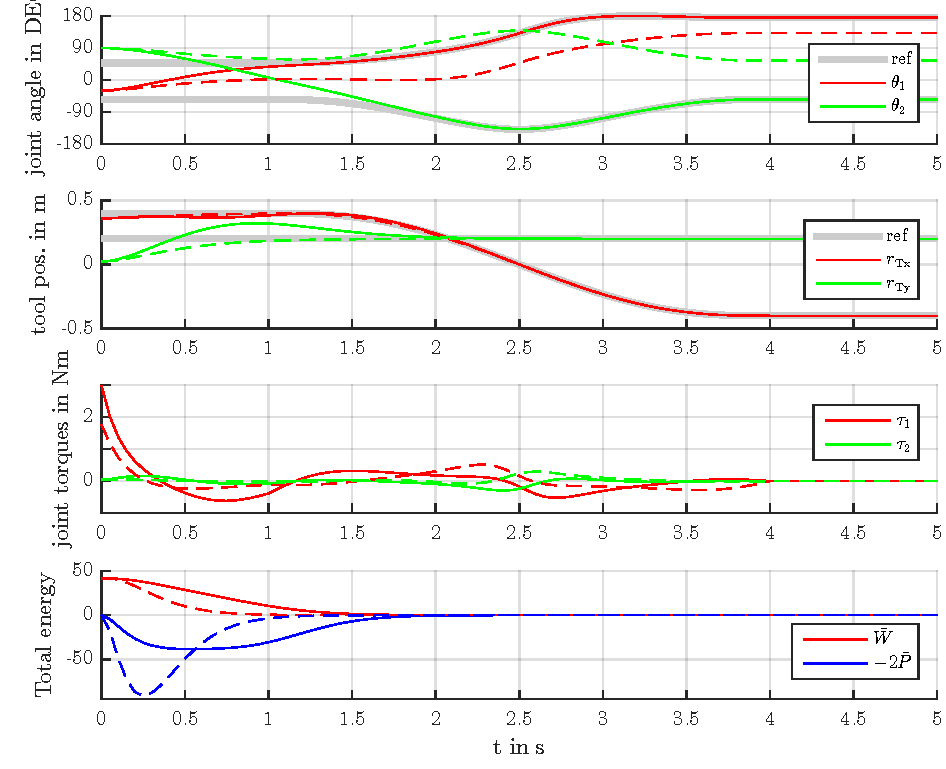
\includegraphics[]{SCARA/ScaraSimRes.pdf}
 \caption{Simulation result for the SCARA with parameterization 1 (solid lines) and 2 (dashed lines)}
 \label{fig:ScaraSimRes}
\end{figure}

\begin{figure}[htb]
 \centering
 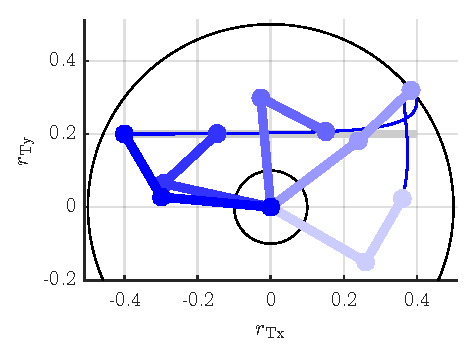
\includegraphics[]{SCARA/ScaraSnapApproach1.pdf}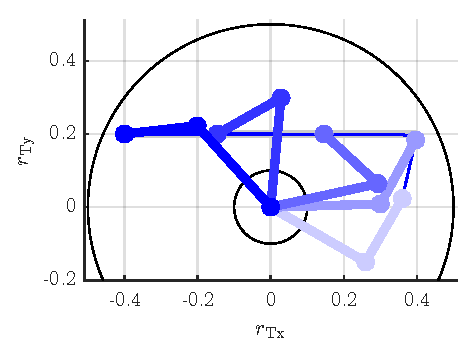
\includegraphics[]{SCARA/ScaraSnapApproach2.pdf}
 \caption{Snapshots for the simulation result for the SCARA with parameterization 1 (left) and 2 (right)}
 \label{fig:ScaraSimSnapshots}
\end{figure}

\begin{figure}[ht]
 \centering
 \input{graphics/SCARAPotential.pdf_tex}
 \caption{
 The controlled potential energy $\potentialEnergy$ for parameterization 1 (left) and 2 (right) for $\jointAngleR[1] = 0$, $\jointAngleR[2] = \tfrac{\pi}{2}$. %on the half open set $\jointAngle[1], \jointAngle[2] = (-\pi,\pi]$.
 Blue dots are minima, red are maxima and green are saddle points.
 }
 \label{fig:SCARAPotentials}
\end{figure}


